\mysubsection{Fabian Gärtner}{Personenerkennung mittels Microsoft Kinect}

Zur Erkennung von Personen auf dem Spielfeld mittels Microsoft Kinect konnten keine Standardfunktionen verwendet werden, da das Kinect-SDK den Einsatz der Kinect aus der Vogelperspektive nicht vorsieht. Stattdessen muss das von der Kinect aufgenommene Tiefenbild mittels Bildverarbeitungstechniken auf Personen bzw. verallgemeinert gesprochen auf Objektkonturen hin untersucht werden. In BlinkenTiles sind dafür die drei Klassen \enquote{KinectManager}, \enquote{BlobDetection} und \enquote{BlobDetectionThread} zuständig. Erstere fragt unter Anwendung des Kinect-SDKs von Microsoft das Tiefenbild (30 Bilder pro Sekunde mit einer Auflösung von 512 x 424 Pixel) und -- bei Bedarf -- das Farbbild (15 Bilder pro Sekunde mit einer Auflösung von 1920 x 1080 Pixel) der Kinect ab. Das Tiefenbild ist dabei ein zweidimensionales Array, das mit Werten zwischen 0 und 8000 die pro Pixel gemessene Tiefe in Millimeter angibt. Da sich die Farbkamera von der Tiefenkamera in Auflösung und Bildwinkel unterscheidet, müssen die Werte des Farbbildes, um beide Bilder übereinander legen zu können, mittels einer vom Kinect-SDK bereitgestellten Funktion umgerechnet werden. Auch diese Funktionalität und die Möglichkeit, Tiefenbilder in Form von Dateien abzuspeichern und für den Fall, dass die Kinect nicht angeschlossen ist, als Testdaten zu verwenden, stellt die Klasse bereit.

Die Weiterverarbeitung des Tiefenbildes und damit die eigentliche Bildverarbeitung findet in der Klasse \enquote{BlobDetectionThread} statt und wird zur Laufzeit in einem eigenen Thread ausgeführt. Dies war zu Beginn der Entwicklung noch notwendig, da die anfangs prozessorlastige Objekterkennung zu einer niedrigen Bildrate in der Hauptanwendung führte und damit auch Auswirkungen auf den Spielablauf und das Abspielen der Musik hatte. Dieser Prozess konnte im Verlauf der Entwicklung aber stetig optimiert werden, sodass die Bildverarbeitung auf eine Dauer von lediglich 12 Millisekunden pro Tiefenbild reduziert werden konnte. Mit etwas mehr als 80 Bildern pro Sekunde liegt die Objekterkennung damit bereits weit über der Bildrate der Kinect mit rund 30 Bildern pro Sekunde und kann ohne Verzögerung und in Echtzeit stattfinden. Die Auslagerung in einen eigenen Thread wurde aber beibehalten, sodass die Arbeitslast auch weiterhin gleichmäßig auf mehrere CPU-Kerne verteilt wird und mögliche Verzögerungen bei der Abfrage der Tiefenbilder keine Auswirkungen auf die Hauptanwendung und den Spielablauf haben.

Hauptsächlich für die Bildverarbeitung verwendet wird die kostenfreie Open-Source-Bibliothek OpenCV, die über den C-Sharp-Wrapper EmguCV angesteuert wird. OpenCV erlaubt die Anwendung von Algorithmen und grundlegenden mathematischen Operationen auf Matrizen und Bilder. Konkret wird bei BlinkenTiles zunächst das als Array vorliegende Bild gefiltert und normalisiert. Die Filterung arbeitet anhand vom Nutzer eingestellter Werte für minimale und maximale Tiefe. Alle Werte über und alle Werte unter diesen Vorgaben werden auf 0 gesetzt, sodass diese die Erkennung nicht weiter stören. In der Praxis kann damit ein stark reflektierender Boden herausgefiltert werden. Die anschließende Normalisierung hilft, den Kontrast des Tiefenbildes zu erhöhen und so die dann folgende Binarisierung des Bildes zu optimieren. Auf das binarisierte Bild wird letztlich die Konturerkennung von OpenCV angewendet, die Objekte ab einer bestimmten Größe erkennt und ein entsprechendes Konturrechteck zurückliefert. Dieses Rechteck kann anschließend mit den Feldern der Matrix abgeglichen werden und bei Überschneidungen zwischen Konturrechteck und einem Feld das Feld aktiviert werden. Jeder dieser Schritte ist vom Nutzer über eine im Folgenden näher erläuterte GUI separat darstellbar und konfigurierbar, um eine optimale Objekterkennung zu ermöglichen. Des Weiteren werden regelmäßig die einzelnen Schritte als Bilder herausgespeichert, sodass sie den Spielern über den Präsentationsbildschirm angezeigt werden können.

Die Klasse \enquote{BlobDetection} schließlich ist hauptsächlich für die Verwaltung der grafischen Benutzeroberfläche (GUI) der Bildverarbeitung und die Verwaltung der eben beschriebenen Klassen zuständig. Dieser Teil der GUI, wie er in Abbildung X auf Seite X dargestellt ist, nimmt die linke Hälfte der gesamten GUI von BlinkenTiles ein und erstreckt sich damit über einen Monitor. Die GUI stellt das Tiefenbild in seiner ursprünglichen Form oder nach einem der zuvor beschriebenen Verarbeitungsschritte, bspw. in binarisierter Form oder mit farbigen Konturrechtecken um erkannte Objekte, dar. Des Weiteren erlaubt die GUI über eine Reihe von Slidern die Einstellung von Filterwerten, Spielfeld- und Feldergröße sowie Spielfeldposition. Ebenso kann ein Raster über dem Tiefenbild dargestellt werden, bei dem alle aktivieren Felder, also alle Felder auf denen Personen erkannt wurden, farbig markiert sind. Um dieses Raster dem vom Beamer erzeugten Spielfeld anzupassen, also um Beamer und Kinect zu synchronisieren, besteht die Möglichkeit eine Überlagerung von Farb- und Tiefenbild anzuzeigen, die dann die Anpassung der Größe und Ausrichtung des Rasters auf dem Tiefenbild mittels der Slider erlaubt. Alle Einstellungen können auch zuvor über die externe Konfigurationsdatei geladen werden.

\subsubsection{Aufgetretene Probleme}

Am Tag der Medien zeigte sich, dass die Tische, auf denen u.\,a. die LED-Scheinwerfer standen, aufgrund ihrer hellen Oberfläche nicht aus dem Tiefenbild herausgefiltert werden konnten und daher ebenfalls als Objekte erkannt wurden. Dies führte dazu, dass Personen, die auf einem der Felder in der Nähe der Tische standen, zusammen mit den Tischen als ein großes Objekt erkannt und dadurch gelegentlich zu viele Felder gleichzeitig aktiviert wurden. Beheben ließe sich das Problem, indem das Tiefenbild vor der weiteren Verarbeitung auf den relevanten Bereich, also auf Spielfeldgröße zugeschnitten wird. Auch hierfür könnten entsprechende Regler in die GUI integriert werden, sodass der Zuschnitt manuell und je nach Bedarf eingestellt werden kann.

Ein weiteres Problem ist die Perspektive, vor allem dann, wenn die Kinect nicht mittig über dem Spielfeld hängt. So funktioniert die Erkennung von Personen, die sich direkt unter der Kinect befinden zwar tadellos, je weiter eine Person aber von der Kinect entfernt ist, desto mehr Felder deckt sie aufgrund der schrägen Aufsicht gleichzeitig ab. Eine kurzfristige Lösung am Tag der Medien war es, die Felder in der Anwendung größer als in der Realität einzustellen. Des Weiteren wird bereits nicht das ganze Feld auf Überschneidungen mit Konturen überprüft, sondern lediglich ein kleinerer (ebenfalls einstellbarer) Bereich in der Mitte der Felder. Um das Problem aber besser zu lösen, wäre entweder eine zweite Kinect oder eine perspektivisch korrekte Berechnung und ein unsymmetrisches Raster notwendig. So könnten bspw. die Felder des Rasters in den Randbereichen vergrößert oder die Tiefenfilterung zu den Rändern hin verstärkt werden, sodass in diesen Bereichen nur noch die Beine von Personen für die Überschneidung relevant sind, nicht aber der Kopf, der möglicherweise ein anderes Felder überdeckt. Welche Methode sich hier am besten eignet, müsste durch weitere Tests herausgefunden werden.

Störend war auch, dass die Einstellungen zwar wie beschrieben aus einer Konfigurationsdatei geladen werden können, die Werte aber momentan noch per Hand eingetragen werden müssen. Interessant neben einem Button zum Speichern der Einstellungen könnte für eine solche Installation daher auch eine automatische Kalibrierung sein, um bei einem Neustart die manuelle Neukonfiguration zu vermeiden. Technisch ließe sich das über ein vom Beamer dargestelltes Testmuster lösen, das von der Bildvearbeitung erkannt wird und das Raster entsprechend dimensionieren und positionieren lässt. Auch die optimalen Werte für die Filterung könnten so automatisiert ermittelt werden.


\newpage

\begin{figure}[htbp] 
  \centering
     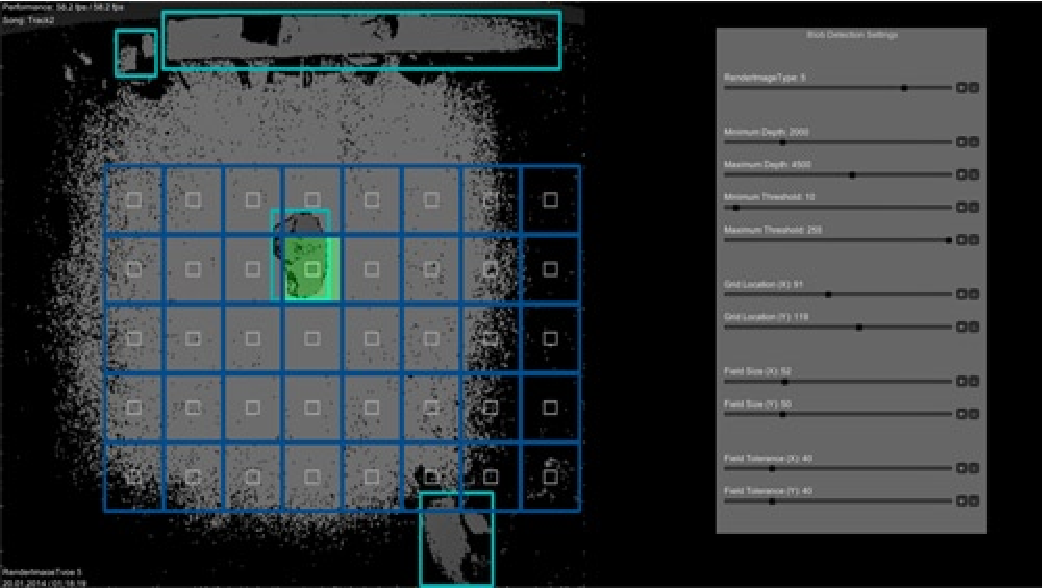
\includegraphics[width=0.9\textwidth]{images/Blob}
  \caption{Schneiden der Spuren in Ableton Live}
  \label{fig:blob}
\end{figure}\todo{caption}